% 'draft' mode can be used to speed up compilation
\documentclass[twoside,final]{hcmut-report}
\usepackage{codespace}

% Encodings
\usepackage{gensymb,textcomp}

% Better tables
\usepackage{array,longtable,multicol,multirow,siunitx,tabularx,booktabs}

% Better enum
\usepackage{enumitem}

% Graphics & TikZ for diagrams
\usepackage{caption,float}
\usepackage[export]{adjustbox}
\usepackage{tikz}
\usetikzlibrary{automata, positioning, arrows.meta, shapes.geometric}

% References
\usepackage[nameinlink]{cleveref}

% Configurations
\coursename{Microprocessors-Microcontrollers}
\reporttype{Lab Report}
\title{Lab 4: Cooperative Scheduler}
% TODO(user): verify the advisor's name
\advisor{& Phan Văn Sỹ &}
\stuname{%
  & Trần Ngọc Bảo & 2452144 \\
}

% Shared TikZ styles for the diagrams
\tikzset{
  st/.style={draw, rounded corners=4pt, minimum width=3.4cm, minimum height=1.3cm,
             align=center, font=\small, thick},
  init/.style={circle, fill, inner sep=1.6pt},
  tr/.style={-{Stealth[length=2.4mm]}, thick},
  lbl/.style={font=\scriptsize, align=center}
}

% Include a figure if the file exists, otherwise show a visible placeholder box
% (so the report still compiles before the screenshots are uploaded)
\newcommand{\figorbox}[3]{%
  \IfFileExists{#1}{\includegraphics[width=#2]{#1}}%
  {\fbox{\parbox{0.8\textwidth}{\centering\vspace{1.5cm}\textbf{TODO(user):} upload \texttt{\detokenize{#1}}\\ #3\vspace{1.5cm}}}}%
}

% Left-aligned paragraph column
\newcolumntype{L}[1]{>{\raggedright\arraybackslash}p{#1}}

% Set depth of numbering for counters
\AtBeginDocument{\counterwithin{lstlisting}{section}}

\begin{document}
\coverpage%

\tableofcontents
\listoffigures
\listoftables
\lstlistoflistings{}

\clearpage

% ============================================================
% SECTION 1 - HARDWARE AND TIMER
% ============================================================
\section{Hardware Design and Timer Configuration}
\subsection{Problem Statement}
Build a test bench for a cooperative scheduler on an STM32F103C6 in Proteus: five LEDs driven by five periodic tasks (0.5~s, 1~s, 1.5~s, 2~s and 2.5~s), one LED driven by a one-shot task, and a serial link that prints a timestamp every time a task runs. A hardware timer must provide a regular 10~ms tick for the scheduler.

\subsection{Proteus Schematic and Pin Mapping}
The circuit (\cref{fig:proteus_schematic}) is built around the STM32F103C6 (U1) and consists of:
\begin{itemize}
    \item \textbf{Six LEDs} (\texttt{LED-RED}). The anodes of D1--D5 are connected to \texttt{Led\_0.5s}, \texttt{Led\_1s}, \texttt{Led\_1.5s}, \texttt{Led\_2s} and \texttt{Led\_2.5s}, and the anode of D6 to \texttt{one\_shot}. All cathodes go to ground, so every LED is \emph{active-high} (a pin driven to logic~1 turns its LED on). The LEDs are driven directly by the GPIO pins, without series resistors, as drawn in the simulation schematic.
    \item \textbf{A Virtual Terminal} connected to \texttt{USART1}: the terminal's \texttt{RXD} is wired to \texttt{USART1\_TX} (PA9) and its \texttt{TXD} to \texttt{USART1\_RX} (PA10). Only the transmit direction is used by the firmware, and \texttt{RTS}/\texttt{CTS} are left unconnected.
    \item \textbf{Power}: +3.3~V on \texttt{VDDA} and ground on \texttt{VSSA}.
\end{itemize}

\begin{table}[H]
    \centering
    \caption{GPIO pin mapping on STM32F103C6}
    \label{tab:pin_mapping}
    \begin{tabular}{llll}
        \toprule
        \textbf{Pin} & \textbf{Net label} & \textbf{Component} & \textbf{Functional role} \\
        \midrule
        PA3  & \texttt{Led\_0.5s} & LED D1 & Periodic task, period 0.5~s \\
        PA4  & \texttt{Led\_1s}   & LED D2 & Periodic task, period 1.0~s \\
        PA5  & \texttt{Led\_1.5s} & LED D3 & Periodic task, period 1.5~s \\
        PA6  & \texttt{Led\_2s}   & LED D4 & Periodic task, period 2.0~s \\
        PA7  & \texttt{Led\_2.5s} & LED D5 & Periodic task, period 2.5~s \\
        PA8  & \texttt{one\_shot} & LED D6 & One-shot task indicator (on for 1~s) \\
        PA9  & \texttt{USART1\_TX} & Virtual Terminal \texttt{RXD} & Timestamp log output \\
        PA10 & \texttt{USART1\_RX} & Virtual Terminal \texttt{TXD} & Not used by the firmware \\
        \bottomrule
    \end{tabular}
\end{table}

\begin{figure}[H]
    \centering
    \figorbox{graphics/proteus_lab4.png}{\textwidth}{Proteus schematic of the Lab 4 test bench}
    \caption{Proteus schematic of the cooperative scheduler test bench}
    \label{fig:proteus_schematic}
\end{figure}

\subsection{STM32CubeIDE Project and Timer Setup}
The MCU runs from the internal HSI oscillator ($f_{\text{clk}} = 8\text{ MHz}$, PLL disabled, all bus prescalers equal to 1). The six LED pins are configured as \texttt{GPIO\_Output} (push-pull, low speed, no pull) and start at logic~0. \texttt{USART1} runs at 57600~bps, 8 data bits, no parity and 1 stop bit (8N1). Timer~2 (\texttt{TIM2}) is the scheduler time base, with $\text{Prescaler (PSC)} = 7999$ and $\text{Counter Period (ARR)} = 9$, and its update interrupt is enabled in the NVIC:
\[
T_{\text{tick}} = \frac{(\text{PSC} + 1) \times (\text{ARR} + 1)}{f_{\text{clk}}} = \frac{8000 \times 10}{8 \times 10^6} = 0.01\text{ s} = 10\text{ ms}
\]
The pin labels in CubeMX are the same net names as in the schematic (\cref{fig:stm32_setup}), so \texttt{main.h} exposes the macros \texttt{Led\_0\_5s\_Pin}, \texttt{Led\_1s\_Pin}, \dots, \texttt{one\_shot\_Pin}. The scheduler is kept in its own module, and the application tasks in another one, so that \texttt{main.c} stays almost unchanged:
\begin{lstlisting}[language={}, caption={Project file organisation}]
Core/Inc:  main.h  app.h  scheduler.h  stm32f1xx_hal_conf.h  stm32f1xx_it.h
Core/Src:  main.c  app.c  scheduler.c  stm32f1xx_it.c  stm32f1xx_hal_msp.c
           system_stm32f1xx.c  syscalls.c  sysmem.c
\end{lstlisting}

\begin{figure}[H]
    \centering
    \figorbox{graphics/stm32_lab4.png}{0.75\textwidth}{STM32CubeMX pinout of the Lab 4 project (PA3--PA10, TIM2, USART1)}
    \caption{STM32CubeMX pinout of the project}
    \label{fig:stm32_setup}
\end{figure}

\subsection{Conclusion}
The hardware provides six independent LED outputs and a serial log, and \texttt{TIM2} produces an exact 10~ms tick ($f = 100$~Hz) from the 8~MHz internal clock. Every scheduler delay and period in this report is therefore an integer number of 10~ms ticks.

% ============================================================
% SECTION 2 - SCHEDULER
% ============================================================
\section{Cooperative Scheduler Implementation}
\subsection{Problem Statement}
Implement a cooperative scheduler in its own source file, with at least the four functions required by the handout: \texttt{SCH\_Update()}, \texttt{SCH\_Dispatch\_Tasks()}, \texttt{SCH\_Add\_Task()} (which returns an ID) and \texttt{SCH\_Delete\_Task()} (which deletes a task by its ID). The handout also lists designs that are considered unsatisfactory: supporting only one timeout at a time, delivering callbacks in the wrong order, and doing $O(n)$ searches inside \texttt{SCH\_Update()}.

\subsection{Design: a Delta List Ordered by Due Time}
A scheduler that stores one counter per task in an array has to visit every slot in \texttt{SCH\_Update()}, and its dispatcher runs tasks in slot order instead of due-time order. To avoid both problems, the tasks are kept in a singly linked \emph{delta list}, sorted by due time, where each node stores only the delay \emph{relative to the node in front of it} (\cref{fig:delta_list}). Only the head of the list is counted down, so the whole list advances with a single decrement per tick.

\begin{figure}[H]
    \centering
    \resizebox{\textwidth}{!}{%
    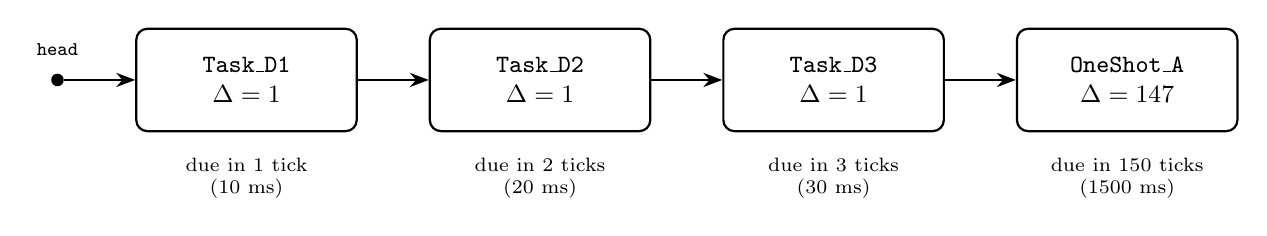
\begin{tikzpicture}
        \node[init] (h0) {};
        \node[lbl, above=1mm of h0] {\texttt{head}};
        \node[st, minimum width=2.8cm, right=0.9cm of h0] (n1) {\texttt{Task\_D1}\\ $\Delta = 1$};
        \node[st, minimum width=2.8cm, right=0.9cm of n1] (n2) {\texttt{Task\_D2}\\ $\Delta = 1$};
        \node[st, minimum width=2.8cm, right=0.9cm of n2] (n3) {\texttt{Task\_D3}\\ $\Delta = 1$};
        \node[st, minimum width=2.8cm, right=0.9cm of n3] (n4) {\texttt{OneShot\_A}\\ $\Delta = 147$};
        \draw[tr] (h0) -- (n1);
        \draw[tr] (n1) -- (n2);
        \draw[tr] (n2) -- (n3);
        \draw[tr] (n3) -- (n4);
        \node[lbl, below=2mm of n1] {due in 1 tick\\ (10 ms)};
        \node[lbl, below=2mm of n2] {due in 2 ticks\\ (20 ms)};
        \node[lbl, below=2mm of n3] {due in 3 ticks\\ (30 ms)};
        \node[lbl, below=2mm of n4] {due in 150 ticks\\ (1500 ms)};
    \end{tikzpicture}}
    \caption{Illustrative delta list: each node stores the delay relative to its predecessor}
    \label{fig:delta_list}
\end{figure}

The work is split between the interrupt and the main loop (\cref{fig:architecture}). The timer interrupt only advances the clock and counts down the head, which keeps it very short; the main loop removes the due tasks from the list and runs them. A long task can therefore never make the scheduler miss a tick.

\begin{figure}[H]
    \centering
    \resizebox{\textwidth}{!}{%
    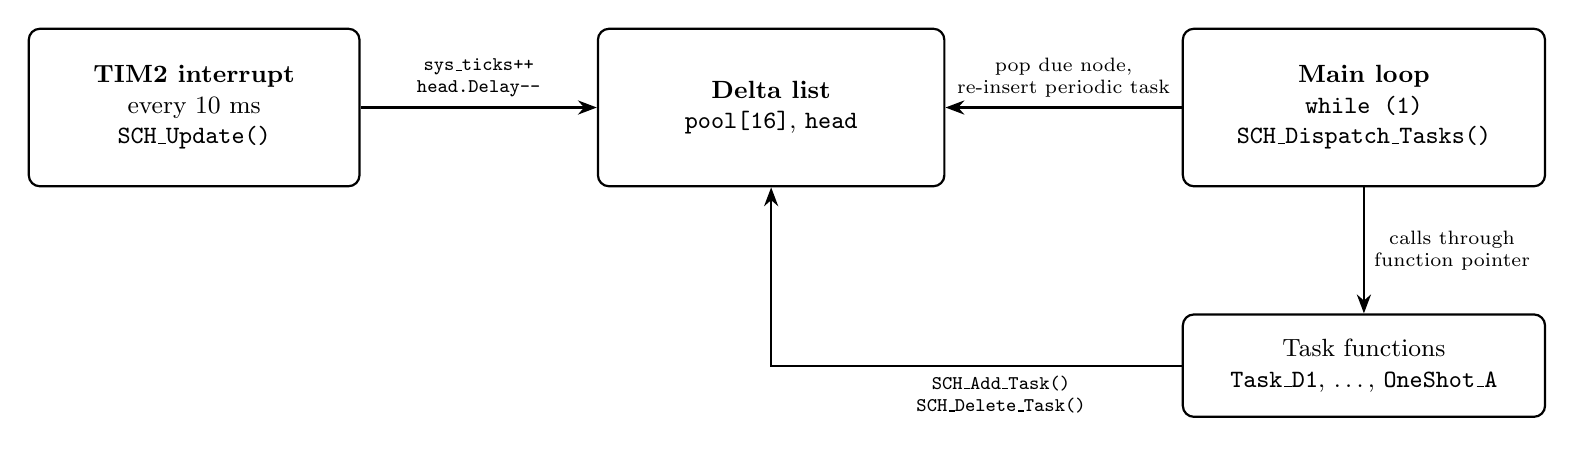
\begin{tikzpicture}
        \node[st, minimum width=4.2cm, minimum height=2cm] (isr) {\textbf{TIM2 interrupt}\\ every 10~ms\\ \texttt{SCH\_Update()}};
        \node[st, minimum width=4.4cm, minimum height=2cm, right=3cm of isr] (list) {\textbf{Delta list}\\ \texttt{pool[16]}, \texttt{head}};
        \node[st, minimum width=4.6cm, minimum height=2cm, right=3cm of list] (main) {\textbf{Main loop}\\ \texttt{while (1)}\\ \texttt{SCH\_Dispatch\_Tasks()}};
        \node[st, minimum width=4.6cm, minimum height=1.3cm, below=1.6cm of main] (tasks) {Task functions\\ \texttt{Task\_D1}, \dots, \texttt{OneShot\_A}};
        \draw[tr] (isr) -- node[above, lbl] {\texttt{sys\_ticks++}\\ \texttt{head.Delay-{}-}} (list);
        \draw[tr] (main) -- node[above, lbl] {pop due node,\\ re-insert periodic task} (list);
        \draw[tr] (main) -- node[right, lbl] {calls through\\ function pointer} (tasks);
        \draw[tr] (tasks.west) -| node[below, lbl, pos=0.22] {\texttt{SCH\_Add\_Task()}\\ \texttt{SCH\_Delete\_Task()}} (list.south);
    \end{tikzpicture}}
    \caption{Division of work between the timer interrupt and the main loop}
    \label{fig:architecture}
\end{figure}

\begin{table}[H]
    \centering
    \caption{Cost of the scheduler operations}
    \label{tab:complexity}
    \begin{tabular}{L{0.28\textwidth}L{0.3\textwidth}L{0.3\textwidth}}
        \toprule
        \textbf{Operation} & \textbf{Cost} & \textbf{Runs in} \\
        \midrule
        \texttt{SCH\_Update()} & $O(1)$ & Timer interrupt (every 10~ms) \\
        \texttt{SCH\_Dispatch\_Tasks()} & $O(1)$ per due task, $O(n)$ to re-insert a periodic task & Main loop \\
        \texttt{SCH\_Add\_Task()} & $O(n)$ (sorted insertion) & Main loop or a task, never the interrupt \\
        \texttt{SCH\_Delete\_Task()} & $O(n)$ (search by ID) & Main loop or a task \\
        \bottomrule
    \end{tabular}
\end{table}

\subsection{Data Structures and Interface}
The scheduler uses a static pool of \texttt{SCH\_MAX\_TASKS} $= 16$ nodes, so no dynamic memory is needed. Each node holds 17 bytes of data (20 bytes with alignment on the Cortex-M3), which gives 320~bytes of RAM for the whole pool. A node is free when its function pointer is \texttt{NULL}. The pool is larger than the number of registered tasks because one-shot nodes are also created at run time by running tasks. \texttt{TICK\_MS} must match the period of \texttt{TIM2}.

\begin{lstlisting}[language=C, caption={Configuration, task node and public interface in scheduler.h}, label={lst:sched_h}]
#define SCH_MAX_TASKS   16   /* pool size: pending tasks + one-shots created at run time */
#define TICK_MS         10   /* timer period (ms); must match PSC/ARR of TIM2 */

#define NO_TASK_ID      0    /* ID 0 = invalid / error */
#define RETURN_NORMAL   0
#define RETURN_ERROR    1

#define ERROR_SCH_TOO_MANY_TASKS      1
#define ERROR_SCH_CANNOT_DELETE_TASK  2
#define ERROR_SCH_NULL_TASK           3

typedef struct {
    void (*pTask)(void);   /* task function: void f(void) */
    uint32_t Delay;        /* DELTA (ticks) relative to the previous node */
    uint32_t Period;       /* repeat period (ticks); 0 = one-shot */
    uint32_t TaskID;       /* unique identifier */
    int8_t   next;         /* index of the next node, -1 = end of list */
} sTask;

void     SCH_Init(void);
void     SCH_Update(void);                 /* called from the timer ISR */
void     SCH_Dispatch_Tasks(void);         /* called from while(1) */
uint32_t SCH_Add_Task(void (*pFunction)(void), uint32_t DELAY, uint32_t PERIOD);
uint8_t  SCH_Delete_Task(uint32_t taskID);
void     SCH_Go_To_Sleep(void);            /* optional low-power hook */
uint32_t get_time(void);                   /* system time in ms (multiple of TICK_MS) */
\end{lstlisting}

\subsection{Initialisation, Update and Sorted Insertion}
\texttt{SCH\_Init()} empties the pool, the list and the error code. \texttt{SCH\_Update()} is the only function called by the interrupt: it increments the tick counter and decrements the delta of the head if it is still positive. The helper \texttt{insert\_sorted()} walks the list, subtracting the deltas it passes, and links the new node at the position where its remaining delay fits; the following node's delta is reduced accordingly so that all later due times stay unchanged. The comparison uses \texttt{>=}, so tasks due at the same instant keep the order in which they were registered (FIFO).

\begin{lstlisting}[language=C, caption={Pool, sorted insertion, SCH\_Init and SCH\_Update in scheduler.c}, label={lst:sched_core}]
static sTask pool[SCH_MAX_TASKS];
static int8_t head = -1;                     /* -1 = empty list */
static uint32_t newTaskID = 0;
static volatile uint32_t sys_ticks = 0;

volatile uint8_t Error_code_G = 0;

static uint32_t Get_New_Task_ID(void) {
    newTaskID++;
    if (newTaskID == NO_TASK_ID) newTaskID++;    /* skip 0 on wrap-around */
    return newTaskID;
}

/* Insert node idx so that it is due 'delay' ticks from NOW.
 * Must be called with interrupts disabled. */
static void insert_sorted(int8_t idx, uint32_t delay) {
    int8_t prev = -1, cur = head;
    while (cur != -1 && delay >= pool[cur].Delay) {   /* '>=' : equal due time -> FIFO */
        delay -= pool[cur].Delay;
        prev = cur;
        cur = pool[cur].next;
    }
    pool[idx].Delay = delay;
    pool[idx].next  = cur;
    if (cur != -1) pool[cur].Delay -= delay;          /* following node keeps its due time */
    if (prev == -1) head = idx; else pool[prev].next = idx;
}

void SCH_Init(void) {
    for (uint8_t i = 0; i < SCH_MAX_TASKS; i++) {
        pool[i].pTask  = 0;
        pool[i].Delay  = 0;
        pool[i].Period = 0;
        pool[i].TaskID = NO_TASK_ID;
        pool[i].next   = -1;
    }
    head = -1;
    sys_ticks = 0;
    Error_code_G = 0;
}

/* Called from the timer ISR every TICK_MS. O(1). */
void SCH_Update(void) {
    sys_ticks++;
    if (head != -1 && pool[head].Delay > 0) pool[head].Delay--;
}
\end{lstlisting}

\subsection{Adding and Deleting Tasks}
\texttt{SCH\_Add\_Task()} finds a free node, stores the task and links it into the list inside a critical section (the previous \texttt{PRIMASK} value is saved and restored, so the function can also be called from a running task). It returns a unique, non-zero task ID, or \texttt{NO\_TASK\_ID} and an error code if the pointer is \texttt{NULL} or the pool is full. \texttt{SCH\_Delete\_Task()} searches the list by ID, unlinks the node and gives its delta back to the next node so the other tasks are not shifted. It returns \texttt{RETURN\_ERROR} for an unknown ID, for instance a one-shot that has already run.

\begin{lstlisting}[language=C, caption={SCH\_Add\_Task and SCH\_Delete\_Task in scheduler.c}, label={lst:sched_add_del}]
uint32_t SCH_Add_Task(void (*pFunction)(void), uint32_t DELAY, uint32_t PERIOD) {
    if (pFunction == 0) {
        Error_code_G = ERROR_SCH_NULL_TASK;
        return NO_TASK_ID;
    }

    int8_t idx = -1;
    for (uint8_t i = 0; i < SCH_MAX_TASKS; i++) {
        if (pool[i].pTask == 0) { idx = (int8_t)i; break; }
    }
    if (idx < 0) {                                    /* pool is full */
        Error_code_G = ERROR_SCH_TOO_MANY_TASKS;
        return NO_TASK_ID;
    }

    uint32_t pm = __get_PRIMASK();
    __disable_irq();
    pool[idx].pTask  = pFunction;
    pool[idx].Period = PERIOD;
    pool[idx].TaskID = Get_New_Task_ID();
    uint32_t id = pool[idx].TaskID;
    insert_sorted(idx, DELAY);
    __set_PRIMASK(pm);
    return id;
}

uint8_t SCH_Delete_Task(uint32_t taskID) {
    if (taskID == NO_TASK_ID) {
        Error_code_G = ERROR_SCH_CANNOT_DELETE_TASK;
        return RETURN_ERROR;
    }

    uint32_t pm = __get_PRIMASK();
    __disable_irq();
    int8_t prev = -1, cur = head;
    while (cur != -1 && pool[cur].TaskID != taskID) {
        prev = cur;
        cur = pool[cur].next;
    }
    if (cur == -1) {                                  /* ID not found */
        __set_PRIMASK(pm);
        Error_code_G = ERROR_SCH_CANNOT_DELETE_TASK;
        return RETURN_ERROR;
    }

    if (pool[cur].next != -1)                         /* give the delta back to the next node */
        pool[pool[cur].next].Delay += pool[cur].Delay;
    if (prev == -1) head = pool[cur].next; else pool[prev].next = pool[cur].next;

    pool[cur].pTask  = 0;
    pool[cur].Delay  = 0;
    pool[cur].Period = 0;
    pool[cur].TaskID = NO_TASK_ID;
    pool[cur].next   = -1;
    __set_PRIMASK(pm);
    return RETURN_NORMAL;
}
\end{lstlisting}

\subsection{The Dispatcher}
\texttt{SCH\_Dispatch\_Tasks()} runs in the super loop. Each pass of its inner loop checks, with interrupts disabled, whether the head is due (\texttt{Delay == 0}). If so, the head is removed from the list. A periodic task is immediately re-inserted with its period, a one-shot node is released, and only then are the interrupts re-enabled and the function called. Three consequences follow from this order:
\begin{itemize}
    \item The task runs with interrupts enabled, so the 10~ms tick keeps being counted while it executes.
    \item A one-shot task can register a new task from inside its own callback, which is how the one-shot LED of \cref{sec:oneshot} is switched off.
    \item Tasks that are due at the same time run one after another in the order of the list, i.e.\ in due-time order.
\end{itemize}
When no task is due, the optional \texttt{SCH\_Go\_To\_Sleep()} can put the CPU to sleep with \texttt{WFI} until the next tick; it is disabled by default (\texttt{SCH\_USE\_SLEEP = 0}). \texttt{get\_time()} converts the tick counter to milliseconds and is used for all timestamps.

\begin{lstlisting}[language=C, caption={SCH\_Dispatch\_Tasks, SCH\_Go\_To\_Sleep and get\_time in scheduler.c}, label={lst:sched_dispatch}]
void SCH_Dispatch_Tasks(void) {
    for (;;) {
        uint32_t pm = __get_PRIMASK();
        __disable_irq();
        if (head == -1 || pool[head].Delay != 0) {    /* no task is due yet */
            __set_PRIMASK(pm);
            break;
        }
        int8_t idx = head;
        head = pool[idx].next;                         /* remove the head from the list */
        void (*fn)(void) = pool[idx].pTask;

        if (pool[idx].Period > 0) {
            insert_sorted(idx, pool[idx].Period);      /* periodic: re-insert BEFORE running */
        } else {                                       /* one-shot: release the node */
            pool[idx].pTask  = 0;
            pool[idx].TaskID = NO_TASK_ID;
            pool[idx].next   = -1;
        }
        __set_PRIMASK(pm);

        fn();                                          /* run the task, interrupts enabled */
    }
    SCH_Go_To_Sleep();
}

void SCH_Go_To_Sleep(void) {
#if SCH_USE_SLEEP
    __WFI();                                           /* sleep until the next tick */
#endif
}

uint32_t get_time(void) {
    return sys_ticks * TICK_MS;
}
\end{lstlisting}

\subsection{Conclusion}
The scheduler consists of the four required functions plus \texttt{SCH\_Init()}, \texttt{SCH\_Go\_To\_Sleep()} and \texttt{get\_time()}. The delta list keeps \texttt{SCH\_Update()} at $O(1)$, delivers callbacks in due-time order and supports many simultaneous timeouts, and the critical sections are limited to a few pointer operations.

% ============================================================
% SECTION 3 - PERIODIC TASKS
% ============================================================
\section{Periodic Tasks}
\subsection{Problem Statement}
The main program must run five tasks periodically, every 0.5~s, 1~s, 1.5~s, 2~s and 2.5~s. Each task toggles its LED and prints a timestamp.

\subsection{Source Code}
All delays and periods are given to \texttt{SCH\_Add\_Task()} in ticks, converted from milliseconds by \texttt{MS2TICK(ms) = (ms) / TICK\_MS}. The helper \texttt{log\_msg()} prints \texttt{[ time ms] text} on \texttt{USART1}, where the time comes from \texttt{get\_time()}, so every timestamp is a multiple of 10~ms. Each LED toggles whenever its task runs, so an LED with a 0.5~s task changes state every 0.5~s (one full blink every 1~s).

\begin{lstlisting}[language=C, caption={Timestamp logging and the five periodic tasks in app.c}, label={lst:periodic_tasks}]
#define LED_PORT   GPIOA
#define PIN_D1     GPIO_PIN_3      /* Led_0.5s */
#define PIN_D2     GPIO_PIN_4      /* Led_1s   */
#define PIN_D3     GPIO_PIN_5      /* Led_1.5s */
#define PIN_D4     GPIO_PIN_6      /* Led_2s   */
#define PIN_D5     GPIO_PIN_7      /* Led_2.5s */
#define PIN_D6     GPIO_PIN_8      /* one_shot */
#define MS2TICK(ms)  ((ms) / TICK_MS)

/* Print "[ time ms] text" on USART1 (Virtual Terminal) */
static void log_msg(const char *text)
{
    char buf[48];
    int n = snprintf(buf, sizeof(buf), "[%6lu ms] %s\r\n",
                     (unsigned long)get_time(), text);
    if (n <= 0) return;
    if (n >= (int)sizeof(buf)) n = (int)sizeof(buf) - 1;   /* output was truncated */
    HAL_UART_Transmit(&huart1, (uint8_t *)buf, (uint16_t)n, 20);
}

static void Task_D1(void) { HAL_GPIO_TogglePin(LED_PORT, PIN_D1); log_msg("0.5s"); }
static void Task_D2(void) { HAL_GPIO_TogglePin(LED_PORT, PIN_D2); log_msg("1.0s"); }
static void Task_D3(void) { HAL_GPIO_TogglePin(LED_PORT, PIN_D3); log_msg("1.5s"); }
static void Task_D4(void) { HAL_GPIO_TogglePin(LED_PORT, PIN_D4); log_msg("2.0s"); }
static void Task_D5(void) { HAL_GPIO_TogglePin(LED_PORT, PIN_D5); log_msg("2.5s"); }
\end{lstlisting}

\paragraph{Avoiding task overlap.} The five periods are multiples of 0.5~s, so without precautions all of them would become due in the same tick at $t = 30$~s (the least common multiple of 500, 1000, 1500, 2000 and 2500~ms), and D1, D2 and D3 would already coincide every 3~s. Tasks that are due together run one after another, so the later ones would be delayed by the earlier ones. The tasks are therefore registered with staggered initial delays of 1, 2, 3, 4 and 5 ticks:
\begin{lstlisting}[language=C, caption={Registration of the periodic tasks in App\_Init()}, label={lst:periodic_reg}]
SCH_Add_Task(Task_D1, 1, MS2TICK(500));    /* 0.5 s */
SCH_Add_Task(Task_D2, 2, MS2TICK(1000));   /* 1.0 s */
SCH_Add_Task(Task_D3, 3, MS2TICK(1500));   /* 1.5 s */
SCH_Add_Task(Task_D4, 4, MS2TICK(2000));   /* 2.0 s */
SCH_Add_Task(Task_D5, 5, MS2TICK(2500));   /* 2.5 s */
\end{lstlisting}
Each task keeps its own offset of 10--50~ms, because a periodic task is re-inserted with exactly its period, so as long as every task finishes within one tick, no two of these tasks share a tick.

\paragraph{Timer interrupt and main loop.} The interrupt callback only calls \texttt{SCH\_Update()}; the super loop only calls the dispatcher.
\begin{lstlisting}[language=C, caption={Timer callback in app.c and super loop in main.c}, label={lst:isr_main}]
/* app.c */
void HAL_TIM_PeriodElapsedCallback(TIM_HandleTypeDef *htim)
{
    if (htim->Instance == TIM2) {
        SCH_Update();
    }
}

/* main.c */
App_Init();                    /* SCH_Init(), register all tasks, start TIM2 */
while (1)
{
    SCH_Dispatch_Tasks();
}
\end{lstlisting}

\subsection{Expected Timeline}
\cref{tab:timeline_periodic} lists the first timestamps printed by each periodic task. They were obtained by running the scheduler source of \cref{lst:sched_core,lst:sched_add_del,lst:sched_dispatch} and the application tasks of this section on a PC with the interrupt replaced by one call of \texttt{SCH\_Update()} per 10~ms tick (task execution time ignored), so they are the theoretical values that the Virtual Terminal should show.

\begin{table}[H]
    \centering
    \caption{Registered parameters and first timestamps of the periodic tasks}
    \label{tab:timeline_periodic}
    \begin{tabular}{lL{0.17\textwidth}L{0.2\textwidth}L{0.33\textwidth}}
        \toprule
        \textbf{Task (LED)} & \textbf{Delay} & \textbf{Period} & \textbf{Timestamps printed (ms)} \\
        \midrule
        \texttt{Task\_D1} (D1) & 1 tick (10 ms) & 50 ticks (500 ms) & 10, 510, 1010, 1510, 2010, 2510, \dots \\
        \texttt{Task\_D2} (D2) & 2 ticks (20 ms) & 100 ticks (1000 ms) & 20, 1020, 2020, 3020, 4020, \dots \\
        \texttt{Task\_D3} (D3) & 3 ticks (30 ms) & 150 ticks (1500 ms) & 30, 1530, 3030, 4530, 6030, \dots \\
        \texttt{Task\_D4} (D4) & 4 ticks (40 ms) & 200 ticks (2000 ms) & 40, 2040, 4040, 6040, 8040, \dots \\
        \texttt{Task\_D5} (D5) & 5 ticks (50 ms) & 250 ticks (2500 ms) & 50, 2550, 5050, 7550, 10050, \dots \\
        \bottomrule
    \end{tabular}
\end{table}

\subsection{Conclusion}
Five periodic tasks run concurrently with exact periods of 0.5, 1, 1.5, 2 and 2.5~s. The timer interrupt contains only \texttt{SCH\_Update()}, and the staggered initial delays prevent the tasks from colliding when their periods coincide.

% ============================================================
% SECTION 4 - ONE-SHOT, DELETE, DEMONSTRATION
% ============================================================
\section{One-Shot Tasks, Task Deletion and Demonstration}
\label{sec:oneshot}
\subsection{Problem Statement}
Besides periodic tasks, the scheduler must support one-shot tasks (\texttt{PERIOD = 0}), deletion by ID, and the demonstration scenario of the handout: a regular 10~ms tick, a callback every 10~ms that prints the value returned by \texttt{get\_time()}, several timeouts registered at the same time, and a few \texttt{SCH\_Add\_Task()} calls made before the main loop with delays long enough for the loop to be entered first.

\subsection{Source Code}
\paragraph{One-shot LED (D6).} \texttt{Task\_D6\_Trigger} is a periodic task (first run at 1.2~s, then every 3~s). On every run it turns D6 on and registers a \emph{one-shot} task, \texttt{OneShot\_D6\_Off}, that fires 1~s later, turns D6 off and is then released by the scheduler. If the pool were full, D6 is turned off immediately so it can never stay on.
\begin{lstlisting}[language=C, caption={Periodic trigger and chained one-shot task for D6 in app.c}, label={lst:oneshot}]
#define D6_TRIGGER_FIRST_MS    1200  /* first trigger of D6 */
#define D6_TRIGGER_PERIOD_MS   3000  /* D6 is triggered again every 3 s */
#define D6_PULSE_MS            1000  /* D6 stays on for 1 s */

static void OneShot_D6_Off(void)
{
    HAL_GPIO_WritePin(LED_PORT, PIN_D6, GPIO_PIN_RESET);
    log_msg("D6 OFF (one-shot)");
}

static void Task_D6_Trigger(void)
{
    HAL_GPIO_WritePin(LED_PORT, PIN_D6, GPIO_PIN_SET);
    log_msg("D6 ON  (+1s one-shot)");
    if (SCH_Add_Task(OneShot_D6_Off, MS2TICK(D6_PULSE_MS), 0) == NO_TASK_ID) {
        /* pool is full: switch off immediately */
        HAL_GPIO_WritePin(LED_PORT, PIN_D6, GPIO_PIN_RESET);
    }
}
\end{lstlisting}

\paragraph{10~ms callback and task deletion.} \texttt{Task\_Tick10} is registered with a delay of 0 and a period of one tick, so it runs as soon as the main loop starts and then every 10~ms, printing the value of \texttt{get\_time()}. Its ID is stored in \texttt{tick10\_id}. After 2~s, a one-shot task calls \texttt{SCH\_Delete\_Task(tick10\_id)} and reports whether the deletion succeeded, which exercises the delete function while other tasks keep running.

\paragraph{Ordering test.} Three one-shot tasks are registered in the order C, B, A, i.e.\ \emph{opposite} to their due times (5~s, 3~s and 1.5~s). A scheduler that delivers callbacks in registration order would print C first; the delta list must print A, B, C. All of them are registered before \texttt{TIM2} is started, with delays far longer than the time needed to enter the main loop.

\begin{lstlisting}[language=C, caption={Demonstration tasks and complete App\_Init() in app.c}, label={lst:app_init}]
static uint32_t tick10_id = NO_TASK_ID;

static void Task_Tick10(void) { log_msg("tick10"); }

/* Uses SCH_Delete_Task: stop the 10 ms callback */
static void Task_StopTick10(void)
{
    if (SCH_Delete_Task(tick10_id) == RETURN_NORMAL) log_msg("tick10 DELETED");
    else                                             log_msg("delete FAILED");
}

static void OneShot_A(void) { log_msg("one-shot A (1.5 s)"); }
static void OneShot_B(void) { log_msg("one-shot B (3.0 s)"); }
static void OneShot_C(void) { log_msg("one-shot C (5.0 s)"); }

void App_Init(void)
{
    SCH_Init();

    /* 5 periodic tasks, staggered initial delays */
    SCH_Add_Task(Task_D1, 1, MS2TICK(500));
    SCH_Add_Task(Task_D2, 2, MS2TICK(1000));
    SCH_Add_Task(Task_D3, 3, MS2TICK(1500));
    SCH_Add_Task(Task_D4, 4, MS2TICK(2000));
    SCH_Add_Task(Task_D5, 5, MS2TICK(2500));

    /* periodic task that spawns the one-shot task of D6 */
    SCH_Add_Task(Task_D6_Trigger, MS2TICK(D6_TRIGGER_FIRST_MS), MS2TICK(D6_TRIGGER_PERIOD_MS));

    /* demo: callback every 10 ms (delay 0 = run immediately), deleted after 2 s */
    tick10_id = SCH_Add_Task(Task_Tick10, 0, MS2TICK(10));
    SCH_Add_Task(Task_StopTick10, MS2TICK(2000), 0);

    /* demo: ordering test, registered in REVERSE order of due time */
    SCH_Add_Task(OneShot_C, MS2TICK(5000), 0);
    SCH_Add_Task(OneShot_B, MS2TICK(3000), 0);
    SCH_Add_Task(OneShot_A, MS2TICK(1500), 0);

    HAL_TIM_Base_Start_IT(&htim2);    /* start the 10 ms tick AFTER all tasks are registered */
}
\end{lstlisting}

\subsection{Expected Timeline}
\cref{tab:timeline_oneshot} gives the expected timestamps of the remaining tasks, obtained with the same method as \cref{tab:timeline_periodic}.

\begin{table}[H]
    \centering
    \caption{Registered parameters and timestamps of the one-shot and demonstration tasks}
    \label{tab:timeline_oneshot}
    \begin{tabular}{lL{0.17\textwidth}L{0.17\textwidth}L{0.3\textwidth}}
        \toprule
        \textbf{Task} & \textbf{Delay} & \textbf{Period} & \textbf{Timestamps printed (ms)} \\
        \midrule
        \texttt{Task\_Tick10}      & 0 ticks & 1 tick (10 ms) & 0, 10, 20, \dots, 1990 (200 lines), then deleted \\
        \texttt{Task\_StopTick10}  & 200 ticks (2000 ms) & 0 (one-shot) & 2000 (\texttt{tick10 DELETED}) \\
        \texttt{OneShot\_A}        & 150 ticks (1500 ms) & 0 (one-shot) & 1500 \\
        \texttt{OneShot\_B}        & 300 ticks (3000 ms) & 0 (one-shot) & 3000 \\
        \texttt{OneShot\_C}        & 500 ticks (5000 ms) & 0 (one-shot) & 5000 \\
        \texttt{Task\_D6\_Trigger} & 120 ticks (1200 ms) & 300 ticks (3000 ms) & D6 ON at 1200, 4200, 7200, \dots \\
        \texttt{OneShot\_D6\_Off}  & 100 ticks, created by the trigger & 0 (one-shot) & D6 OFF at 2200, 5200, 8200, \dots \\
        \bottomrule
    \end{tabular}
\end{table}

\begin{figure}[H]
    \centering
    \figorbox{graphics/terminal_lab4.png}{0.8\textwidth}{Screenshot of the Virtual Terminal showing the timestamps (first 6 seconds)}
    \caption{Virtual Terminal output during the Proteus simulation}
    \label{fig:terminal}
\end{figure}

\begin{table}[H]
    \centering
    \caption{Demonstration requirements of the handout and how they are met}
    \label{tab:demo}
    \begin{tabular}{p{0.38\textwidth}p{0.52\textwidth}}
        \toprule
        \textbf{Requirement} & \textbf{Implementation} \\
        \midrule
        A regular 10~ms timer tick & \texttt{TIM2}, PSC = 7999, ARR = 9 at 8~MHz; \texttt{SCH\_Update()} in the update interrupt \\
        A timeout that fires a callback every 10~ms and prints \texttt{get\_time()} & \texttt{Task\_Tick10}, period 1 tick; 200 timestamps from 0 to 1990~ms \\
        More than one timeout registered at a time, with a different interval from the 500~ms one & The five periodic tasks (0.5--2.5~s), \texttt{Task\_D6\_Trigger} (3~s) and \texttt{Task\_Tick10} (10~ms) run concurrently \\
        \texttt{SCH\_Add\_Task} calls before the main loop, with delays long enough for the loop to be entered first & One-shots A, B and C (1.5, 3 and 5~s) are registered in \texttt{App\_Init()}, before \texttt{while (1)}; each only prints its timestamp \\
        Callbacks delivered in the right order & C, B, A are registered in reverse order but are printed as A (1500~ms), B (3000~ms), C (5000~ms) \\
        Every function of the interface is used & \texttt{SCH\_Init}, \texttt{SCH\_Add\_Task}, \texttt{SCH\_Update}, \texttt{SCH\_Dispatch\_Tasks} and \texttt{SCH\_Delete\_Task} (deleting \texttt{Task\_Tick10}) \\
        Timestamps accurate to 10~ms & \texttt{get\_time()} $=$ tick counter $\times$ 10~ms, so every value is a multiple of 10~ms \\
        \bottomrule
    \end{tabular}
\end{table}

\subsection{Conclusion}
One-shot tasks, deletion by ID and one-shot tasks created from inside a running task all work together with the periodic tasks. The ordering test shows that callbacks are delivered by due time and not by registration order.

% ============================================================
% SECTION 5 - EVALUATION
% ============================================================
\section{Final Integration and Evaluation}
\subsection{Problem Statement}
Check the finished system against the designs that the handout calls unsatisfactory, and state the limits of the implementation.

\subsection{Evaluation}
\begin{table}[H]
    \centering
    \caption{Evaluation against the unsatisfactory designs listed in the handout}
    \label{tab:criteria}
    \begin{tabular}{p{0.34\textwidth}p{0.56\textwidth}}
        \toprule
        \textbf{Unsatisfactory design} & \textbf{This implementation} \\
        \midrule
        Only one timeout registered at a time & The pool holds 16 tasks. The demo registers 11 tasks at start-up and has at most 12 active at the same time (when D6 is on and its one-shot is pending) \\
        Callbacks delivered in the wrong order & The list is sorted by due time, with FIFO order for equal due times; the C--B--A test prints A, B, C \\
        $O(n)$ searches in \texttt{SCH\_Update()} & \texttt{SCH\_Update()} increments one counter and decrements one delta, $O(1)$. The $O(n)$ sorted insertion happens only in \texttt{SCH\_Add\_Task()} and when a periodic task is re-inserted, both in the main context \\
        \bottomrule
    \end{tabular}
\end{table}

\subsection{Limits of the Implementation}
\begin{itemize}
    \item \textbf{Time resolution.} Delays and periods are multiples of 10~ms, and \texttt{MS2TICK()} truncates other values.
    \item \textbf{Blocking logging.} \texttt{HAL\_UART\_Transmit()} blocks until the line is sent. At 57600~bps a 20-character line takes about 3.5~ms and a 36-character line about 6.3~ms. Tasks are cooperative and cannot be pre-empted, so a task must finish well inside one tick (10~ms), otherwise the tasks behind it run late. A higher baud rate, or interrupt or DMA transmission with a buffer, would remove this limit.
    \item \textbf{Due tasks are counted only after dispatch.} While the head of the list is due but has not been dispatched yet, the ticks that elapse are not subtracted from the next node. A task running longer than one tick therefore delays the tasks behind it.
    \item \textbf{Pool size.} At most 16 tasks can be pending, and the node index is an \texttt{int8\_t}; \texttt{SCH\_MAX\_TASKS} must stay below 128.
\end{itemize}

\subsection{Project Links}
\begin{itemize}
    % TODO(user): replace with your real links
    \item \textbf{GitHub Repository:} \href{https://github.com/TranNgocBao1/Lab4-Microprocessors-Microcontrollers}{STM32 Source Code and Proteus Simulation}
\end{itemize}

\subsection{Conclusion}
The cooperative scheduler meets the handout: a 10~ms tick, the four required functions with ID-based add and delete, five periodic tasks with periods from 0.5 to 2.5~s, one-shot tasks, and a timestamped log. Its main design choice, the sorted delta list, makes the interrupt $O(1)$, delivers callbacks in the right order and supports several simultaneous timeouts.

% ============================================================
% LAB INFORMATION
% ============================================================
\section*{LAB INFORMATION}
\addcontentsline{toc}{section}{LAB INFORMATION}
Course: Microprocessors-Microcontrollers \\
Course Code: CO3010 \\
Lab 4: Cooperative Scheduler \\
% TODO(user): replace with your real repository link
GitHub Repository: \href{https://github.com/TranNgocBao1/Lab4-Microprocessors-Microcontrollers}{Complete Lab 4 Source Code and Proteus Projects} \\

\end{document}
